\phantomsection
\addcontentsline{toc}{chapter}{Layintroduction}
\chapter*{Layintroduction}

\textit{This section is for all the family, friends, and strangers who have ever
asked me what it is that I actually do, only to come away more confused than
before.}

Welcome! Thanks for opening up my thesis. I'm aware that most people reading
this will never make it past the introduction, and a number will never really
make it through the introduction. (That's okay---I get stuck at the introduction
more often than not too.) These first two-and-a-half pages are a race to sneak
you an impression of my goals for this thesis before the covers are closed. 

Every thesis starts with a question. The question here, in the vague form that
occupies my dreams, is simply `Why do we use diagrams?'. More precisely, I'm
after an `algebra of interconnection' (see the title). Whatever that means.
(Read on to find out $\ddot\smile$.)

Every thesis has a field, and this field tells us what an answer looks like. The
field of this thesis is mathematics. I won't try to make my question more
precise here, but let me quickly say a few words about what the answer looks
like. This is what I hear the cab-driver ask when she says `How do you do
research in mathematics? Isn't it all solved already?'.

In my corner of mathematics the main theme is abstraction and unification. Let
me tell a quick history lesson my supervisor John Baez once told me, from the
very beginning of mathematics. How did we invent number systems?

With civilization came trade, and with trade a need for writing down numbers.
By the 4th millennium BCE, Sumerian innovators had responded admirably to this
task, and many bureaucrats were now skilled in drawing up contracts trading
livestock, or sheaves of wheat, or jars of oil. But there was a problem: each
community had arrived at different ways to represent numbers. So the man
experienced in trading wheat had no ability to describe quantities of cows. It
took another thousand years to unify these systems into single concept of 

This looked like this.\footnote{You can read more about this here.}

Finding the right representation took us all many more years, but was important:
the Arabic system is much easier for many purposes (try to describe addition or
multiplication!) than the Roman system (I, II, III, IV, V) or the Chinese system
(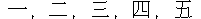
\includegraphics{pics/chinesenumerals}) among others.

By now this is a pattern we mathematicians know well. The central thesis of this
thesis is that certain types of diagrams are just the same. In the abstract I
mentioned some of these types. What is their unified framework? 

Language. networks have `words' (like a battery or resistor), and a `grammar':
this is a well-formed circuit diagram, while this is not. Networks also have
meaning: each well-formed circuit diagram can be understood as, well, a circuit.
So part of this project is a linguistic one, in this sense.

The dream here is to contribute to the invention of richer reasoning systems in
the same vein.

Why bother to do this? Because I really enjoy it: it's fun to understand and
beautiful to see how things fit together. (I hope those who read further agree!)
But I'm optimistic that once we understand why we choose to represent certain
things as networks, and how all our different 

Let me conclude with three different perspectives on where this might lead:

\begin{itemize}
  \item Mathematical physicist Eugene Wigner once described an unreasonable effectiveness of mathematics (see
citation). Biologists hardly feel the same.
Why? Reductionist themes in science and mathematics. Networks and interconnection are better suited to biology.

\item Causal thinking. 
People really like functions. They are causal, they are operational, they situate ourselves in the mathematics: if we do this, then that will happen. Input--output. They are also unphysical. Russell, Willems, Dijkstra have all been skeptical of causality. So what do we do? Relations.

\item Where will it go? Formal tools for reasoning about systems and their
  interconnection.  richer structures for interconnection, and reasoning about
  interconnection Programming. The pioneering computer scientist E.\ W.\
  Dijkstra: languages are too easy to write, not easy enough to read. Coding is
  99\% debugging. \footnote{Citation On the cruelty of really teaching computer
  science.}
\end{itemize}

But we must take small steps towards these grand ideas. What follows is just one
small contribution.

Lastly, some credit to Piper Harron\footnote{This is her blog: . You can find
  her thesis there too, but details are also in the back \cite{Har15}} and her delightful
thesis---this `layintroduction' is inspired by her `laysplanations'. While
technical language and writing has its place (see the rest of this thesis), so
too does nontechnical, accessible writing. I think it's also worth acknowledging
that despite the (hopefully) polished final product, and alongside some years of
fun, awe, and wonder, this thesis has also been the result of years of
procrastination, inadequacy, and blank stares. While I will refrain from a
running commentary on mathematical culture in my thesis, let me echo Piper:
mathematics is a human activity that we are all capable of, and in a better
world technical details and jargon and bad experiences would not scare us all
away. The key ingredients to understanding are curiosity, patience, and
perseverence, not special gifts to a special few. Smash the cult of genius! 

